\chapter{ユーザスタディ}
\label{chap:visualize}

本章では開発したスマートフォンアプリDreamDateの実験方法(調査対象・観察方法)と実験結果ついて説明する。最後に考察を述べた。

\section{予備実験1:音刺激の有無}
 寝る前の10分間とREM睡眠中に音楽を流すことで、夢に影響を与えるか否かを明らかにするために予備実験に取り組んだ。またスマートフォンは充電をした状態で枕の横に置いてもらうことで、音が脳に届く状態にした。また睡眠を始める前に海の夢が見たいと被験者に念じてもらった。\\
 20代後半女性の被験者A、40代後半女性の被験者Bと、20代前半女性の被験者Cに何も音楽を流さない場合と流した場合の結果の違いを分析した。海の音を聞く日と効かない日を交互に14日間続けた。そうすることで、音が夢に影響を与えるのか否かの分析を行った。14日間の実験を行ったのは、睡眠に関する実験は体調、その日の活動内容や、被験者の心境によって左右され、データーが変動しやすいためである。図\ref{experiment1}が実験スケジュールと実験結果である。青のハイライトがある日が夢を見た日だ。\\
 夢の具体的な内容について実験後インタビューをした。すると3日間夢を見たと答えた被験者Aは、音のインプットが無い日は会社で働いている夢を見ることが多く、音を流しながら寝た日は10日ほど前に行った沖縄旅行での夢を見たと答えた。一度も海に関連した夢を見なかった被験者Bは、海の音で起こされたりしたため、音は流れていたが全く関係の無い夢を見たと答えた。被験者Cは実験の最後の方で1年前に旅行したアメリカ西海岸に関する夢を見たと答えた。\\
 結果に個人差が見られたが音が無い場合に被験者が海の夢を見たのは1回なのに対し、海の音を流して海の音を見たのは4回であった。この結果は音が夢にある程度の影響を持っていることを示唆する。また音の影響によってユーザーが起きてしまう事態が発生することが分かった。

\begin{figure}[htbp]
\begin{center}
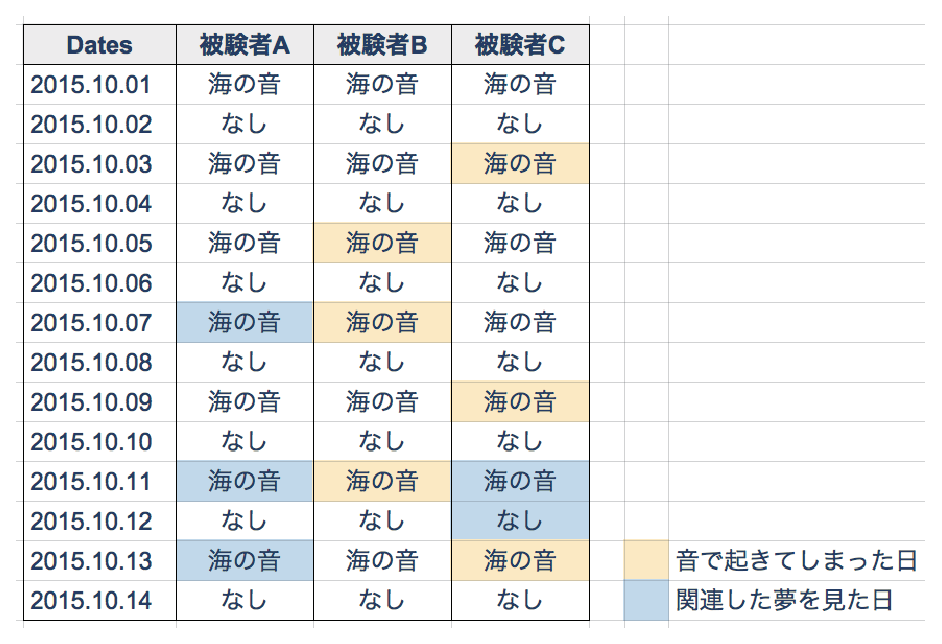
\includegraphics[width=13cm]{eps/schedule0.eps}
\caption{予備実験1:実験スケジュールと実験結果}
\label{experiment1}
\end{center}
\end{figure}

\section{予備実験2:音刺激の種類}
 どのような音がDreamDateで使用するのに適しているのかを調べるために予備実験を行った。遠距離恋愛中の交際相手とデートをしている夢を見たいと望む被験者Cに、「音声」「曲」と「自然音」の3種類の音を試した。被験者Cの場合は「音声」は交際相手が被験者Cの名前を語りかけ、思い出のデートの内容について話している声。「曲」は交際相手が被験者Cのために作曲と演奏した曲。「自然音」はアメリカ西海岸の海で交際相手と共に聞いた波の音。図\ref{experiment2}が実験スケジュールと実験結果である。
 夢の具体的な内容について、実験後インタビューをした。関連する夢を見たのは「曲」と「自然音」のときである。11月9日は日本で再開する夢をみて、11月13日は江ノ島で友人と遊ぶ夢をみた。11月15日は交際相手から手紙が届く夢を見た。\\
 実験の結果から語りかけ口調の音声は被験者を起こしてしまう確率が非常に高い。比べて波の音などの自然音や音楽は比較的被験者を起こす確率が低い。被験者の希望であった遠距離恋愛中の交際相手とデートしたいという要望を実現させることができたのは「曲」であった。

\begin{figure}[htbp]
\begin{center}
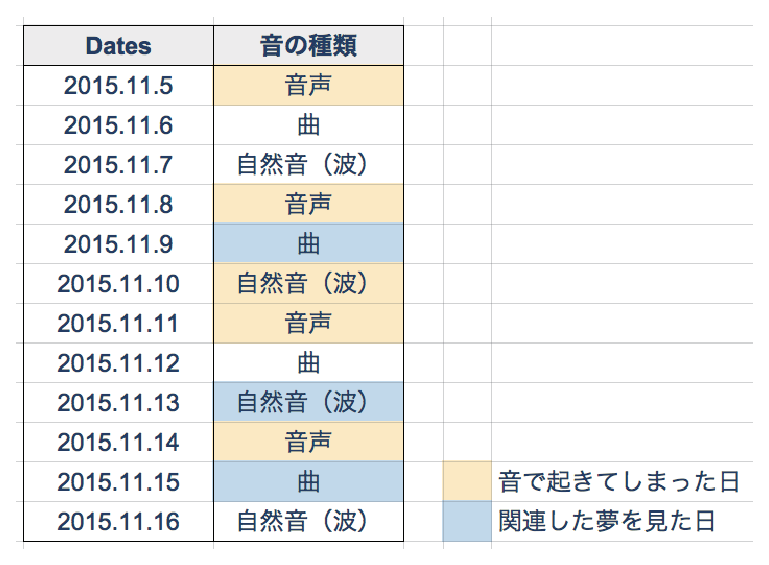
\includegraphics[width=13cm]{eps/schedule1.eps}
\caption{予備実験2:実験スケジュールと実験結果}
\label{experiment2}
\end{center}
\end{figure}

\section{実験:音刺激のタイミング}
 音を流すタイミングによって、夢の結果が変わるのかについて調べるために7人の被験者に15日間の実験に参加してもらった。

\subsection{実験方法}
 被験者にはThe MILD Techniqueに基づいて夢を記憶できる体質になってもらうために実験を開始する5〜10日間前から、被験者には夢日記を書いてもらった。加えて、寝る前に音楽を聴きながら思い出に関する画像を2分間眺めること、思い出について考えならが寝る意識をしてもらった。また6時間以上睡眠を取れる日にのみ実験に臨んでもらった。詳しい事件内容は以下に述べる。実験は1日目は音楽なし、2日目はREM睡眠中音楽あり、3日目は起きる直前のREM睡眠中音楽ありというを繰り返し5回、合計15日間続けてもらった。

\subsection{被験者の詳細}
20歳〜50歳の男女、明晰夢に興味がある7人に参加してもらった。DreamDateは日本人のみならず、全世界のユーザーを対象として制作しているので、国籍と性別共に多様性のある被験者を選んだ。また比較的安定したの睡眠活動をしている人を対象にした。下記に具体的な被験者の情報と使用する音を提示する。

被験者1:
\begin{itemize}
\item 国籍:インドネシア人
\item 性別:男性
\item 年齢:30代後半
\item 明晰夢の経験:5回ほど経験している
\item 夢日記を行ったか否か:5日間行った
\item 思い出に由来する音楽:被験者1は音楽にあまり関心がなく、特に思い出に残る音・音楽がなかった。そこで日常生活の中で音の刷り込みをした。具体的には、実験10日間前から毎日コーヒーを飲むときにEdith Piafによる"Non je ne regrette rien"という曲。この音楽は映画inceptionの中で夢から覚めるために主人公たちが聴く音楽としても知られている。

\end{itemize}
被験者2:
\begin{itemize}
\item 国籍:日本人
\item 性別:女性
\item 年齢:40代後半
\item 明晰夢の経験:経験したことなし
\item 夢日記を行ったか否か:10日間行った
\item 思い出に由来する音楽:被験者2は30年ほど前の結婚式で流した音楽 The CarpentersによるWe've only just begun
\end{itemize}

被験者3:
\begin{itemize}
\item 国籍:日本人
\item 性別:男性
\item 年齢:50代前半
\item 明晰夢の経験:経験したことなし
\item 夢日記を行ったか否か:10日間行った
\item 思い出に由来する音楽:被験者3は007の映画を体験したいということだった。映画の中で使われているサウンドトラック
\end{itemize}

被験者4:
\begin{itemize}
\item 国籍:アメリカ人
\item 性別:男性
\item 年齢:20代前半
\item 明晰夢の経験:5回以上経験したことがある
\item 夢日記を行ったか否か:5日間行った
\item 思い出に由来する音楽:被験者4は宮崎駿の映画である「魔女の宅急便キキ」を体験したいということだった。映画の中で使われているサウンドトラック
\end{itemize}

被験者5:
\begin{itemize}
\item 国籍:日本人
\item 性別:女性
\item 年齢:20代後半
\item 明晰夢の経験:経験したことない
\item 夢日記を行ったか否か:5日間行った
\item 思い出に由来する音楽:被験者5は今年の9月に社会人ダンス部でダンスを披露したときに利用したCell Block Tangoという曲
\end{itemize}

被験者6:
\begin{itemize}
\item 国籍:アメリカ人
\item 性別:男性
\item 年齢:20代前半
\item 明晰夢の経験:何度か経験したことがある
\item 夢日記を行ったか否か:5日間行った
\item 思い出に由来する音楽:高校時代に演奏したバンドの曲、Fountains of WayneによるStacy's Momという曲
\end{itemize}

被験者7:
\begin{itemize}
\item 国籍:アメリカ人
\item 性別:男性
\item 年齢:20代後半
\item 明晰夢の経験:5回以上経験したことある
\item 夢日記を行ったか否か:5日間ほど行った
\item 思い出に由来する音楽:交際相手のために作曲・演奏した曲Love From The Other Side Of The World\end{itemize}

\subsection{実験結果}
図\ref{experiment3}これが実験のスケジュールと実験結果で、図\ref{result}は音楽を流したタイミング別に結果を表した実験結果である。実験の結果から全ての被験者の実験結果を合計し、タイミング別に関連した夢を見たときの確率を導き出した。音を流さないときは1/35、REM睡眠中ずっと音を流したときは10/35、そしてREM睡眠中に夢を見たときは13/35の確率で関連する夢を見た。加えて睡眠中に音楽を流すことで3人の被験者が途中で起きてしまい、睡眠を害してしまった。
\begin{figure}[htbp]
\begin{center}
\includegraphics[width=15cm]{eps/schedule2.eps}
\caption{実験スケジュールと実験結果}
\label{experiment3}
\end{center}
\end{figure}

\begin{figure}[htbp]
\begin{center}
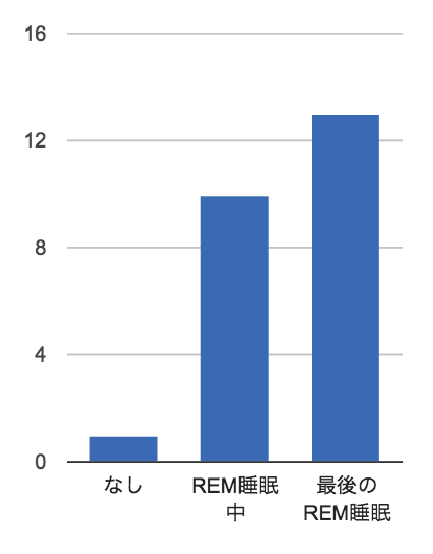
\includegraphics[width=6cm]{eps/result.eps}
\caption{刺激提示のタイミング別の関連した夢を見た回数}
\label{result}
\end{center}
\end{figure}

%丁寧に考えた結果を文章を練り上げて書くこと。	
\section{ユーザスタディの考察}

本研究の実験は全体的に被験者の数が少ないため説得力のあるデータを収集することはできなかった。但し実験を通して明晰夢制御システムの開発にあたって意識するべき様々なポイントを発見できた。\\

予備実験1を通して睡眠中に音で刺激を与えることで明晰夢はある程度誘発できるということがわかった。3人の被験者に海の波の音を睡眠前とREM睡眠中に流した際に2人が海に関連する夢を見た。図\ref{experiment1}を参照。\\

実験を行った後にそれぞれの被験者にどのような夢を見たかインタビューをした。すると海の夢を見た被験者Aと被験者Cはどちらも過去に海に行った際の思い出を夢見たと答えた。一方で海にしばらく行っていない被験者Bは一度も海の夢を見なかった。この結果は被験者の記憶と関連性の高い音を流すと効果が出やすいということが示唆する。言い換えると印象に残っていない体験や情景をDreamDateを使って夢で再現することは極めて困難であるということだ。\\

Zhang Jieは夢は記憶の整理をするために見るものだと述べている\cite{Zhang}。被験者Aの場合波の音が過去の記憶を思い出させる音を流すことがトリガーとなり、脳が反応し思い出が夢として再生されたと考えられる。第2章で紹介したDreamOn、ユメミールやDreamDreamなどのスマートフォンアプリケーションは「鳥の音で森林にいる夢をみることができる」、「貨幣が落ちる音でお金持ちになる夢をみることができる」、「拍手の音で表彰される夢をみることができる」、「フライパンでベーコンが焼ける音で朝食の夢をみることができる」と書いてある。しかしユーザーはそれぞれ違った経験の持ち主なので全てのユーザーにその効果が現れるかは非常に疑い深い。株式会社タカラトミーのホームページでも夢見工房の効果に関しては個人差があると紹介している。その理由もユーザーによって音や香りとそれまでの記憶との関連性が違うからだと推測することができる。\\

予備実験1を経て睡眠中扱う音が結果の有無を左右することが分かった。登録する音ははそれぞれのユーザーに効果の出やすい音を自分で考えて登録してもらう必要性がある。その後に行った実験ではユーザーに前もって音を選んでもらって実験を行った。実験結果によると、自ら作曲した歌、演奏した曲、ダンスをした曲などの直接的な記憶にを連想させる音楽を流した被験者5・6・7は比較的高い確率で関連性のある夢を見た。一方実際に自分は体験していないが映画などを通して間接的に体験した記憶にまつわる音楽を流した被験者3・4はあまり関連性のある夢をみることはできなかった。図\ref{experiment3}を参照。この結果は、流す音がユーザーにとって直接的な体験ほど夢に影響を与えやすいということを示唆している。\\

しかし全ての人が思い出とうまく連携した音を考え付くわけではない。そこで最後に行った実験では被験者1に日常生活の中でコーヒーを飲む時に必ず特定の音楽を聴く習慣をつけてもらうことにした。すると図\ref{experiment3}でもあるように実験の最終日でその夢を見ることができた。Ivan Pavlovは条件反射という考え方を提唱している\cite{pavlov}。Pavlovは実験の中で犬に餌を与える前に決まってサイレンを鳴らし続けた結果、サイレンを鳴らすと犬の唾液量が増える現象が起きたと説明している。犬がサイレンを聞くと餌のことを反射的に考えたためだというのが通説だ。被験者1は最後の夜に一度夢を見ただけのため、被験者の人数を増やしてさらに精度を上げた実験をする必要があるが、REM睡眠中に音楽が鳴ったことで被験者1に条件反射が働きコーヒーを飲む夢を見た可能性があると考えれる。もし仮説が正しければ、旅行をするときに特定の曲を意識的に繰り返し聴くことで旅行が終わった後もDreamDateでその音を流し旅行での想い出を夢で再生することが可能になる。但し、ある夢を見るために生活のあり方を変えるのは相当高いモチベーションを持ったユーザーに限られるだろう。\\

これらの結果から明晰夢における限界を知ることができた。エンジニアリンング力のないユーザーでも比較的気軽に始められるこという利点はあるが、HMDのように空を飛んでいる体験やサイエンス・フィクションなどの近未来的な体験をすることはできない。ただ実験の中で被験者3と被験者4は好きな映画に関連した夢を見ることができたので、サイエンス・フィクションの映画を多く見ることで似た体験ができる余地もある。さらなる実験をする価値はありそうだ。\\

予備実験2で被験者Cは希望であった遠距離恋愛中の交際相手とデートしたいという要望を実現させることができた。被験者Cは物理的制約を超えて交際相手から手紙が届く夢やデートしている夢を見ることで幸せな気持ちを味わうことができた。しかし起床後現実は違うということを悟り少し切ない気持ちを味わってしまったとも答えていた。DreamDateがユーザーに与える心理的影響に関して実験を重ねていく必要があるだろう。\\

予備実験2では効果の現れやすい音を探るために「音声」「曲」「自然音」の3つがそれぞれ与える影響を比較した。もっとも効果が現れたのは交際相手が被験者のために製作した曲を聴いた夜であった。一方で交際相手に名前を呼ばれたり、語りかけられている音声を流した夜は音刺激により起こされて睡眠を害されてしまった。図\ref{experiment2}を参照。この結果かは語りかけ口調の音声はユーザーを起こしてしまうということが分かった。その後、睡眠中のインプットは曲や波や森林などの自然音が好ましいと判断しその後のDreamDateの実験を重ねた。しかし音声でも語りかけ口調ではなく、説明口調出会ったり、歌っている声であったり、考えられる声の種類もたくさんあるので、様々な種類の声で実験を再度行うべきである。その実験はより幅のあるコンテンツを夢で体験することを可能にし、明晰夢システムの開発にとって意義があると考えられる。\\

予備実験の後に行った実験では音をインプットするタイミングとしては、REM睡眠中ずっとではなく音を流すのは起きる直前のREM睡眠の時が最適であるということが判明した。なぜならば最後のREM睡眠時に音を流すだけでもREM睡眠中ずっと音を流すのと同じ効果が見られたからである。図\ref{result}を参照。REM睡眠中は脳が覚醒していて、ユーザーがもっとも起きやすいとされている\cite{remNonRem}。よってユーザーの睡眠が害される可能性を低めるために起きる直前のREM睡眠のみに音を流すが良いだろう。\\